\documentclass[11pt,letterpaper]{exam}
\usepackage[latin1]{inputenc}
\usepackage[left=3.00cm, right=3.00cm, top=3.00cm, bottom=3.00cm]{geometry}% You can change margins here
\usepackage{amsmath}
\usepackage{amsthm}
\usepackage[]{algorithm2e}
\usepackage{amssymb} % use for therefore
\usepackage{tabto}
\usepackage{gensymb}
\usepackage{graphicx} % resize table

\author{Elvric Trombert\\260673394}% Put your Student ID here
\title{Assignment 1 ECSE 420}
\begin{document}
	\maketitle
	\header{Assignment 1 ECSE 420}{}{Elvric Trombert 260673394}
	\hrulefill
	\begin{questions}
		\question
			.
			\begin{figure}[h!]
				\centering
				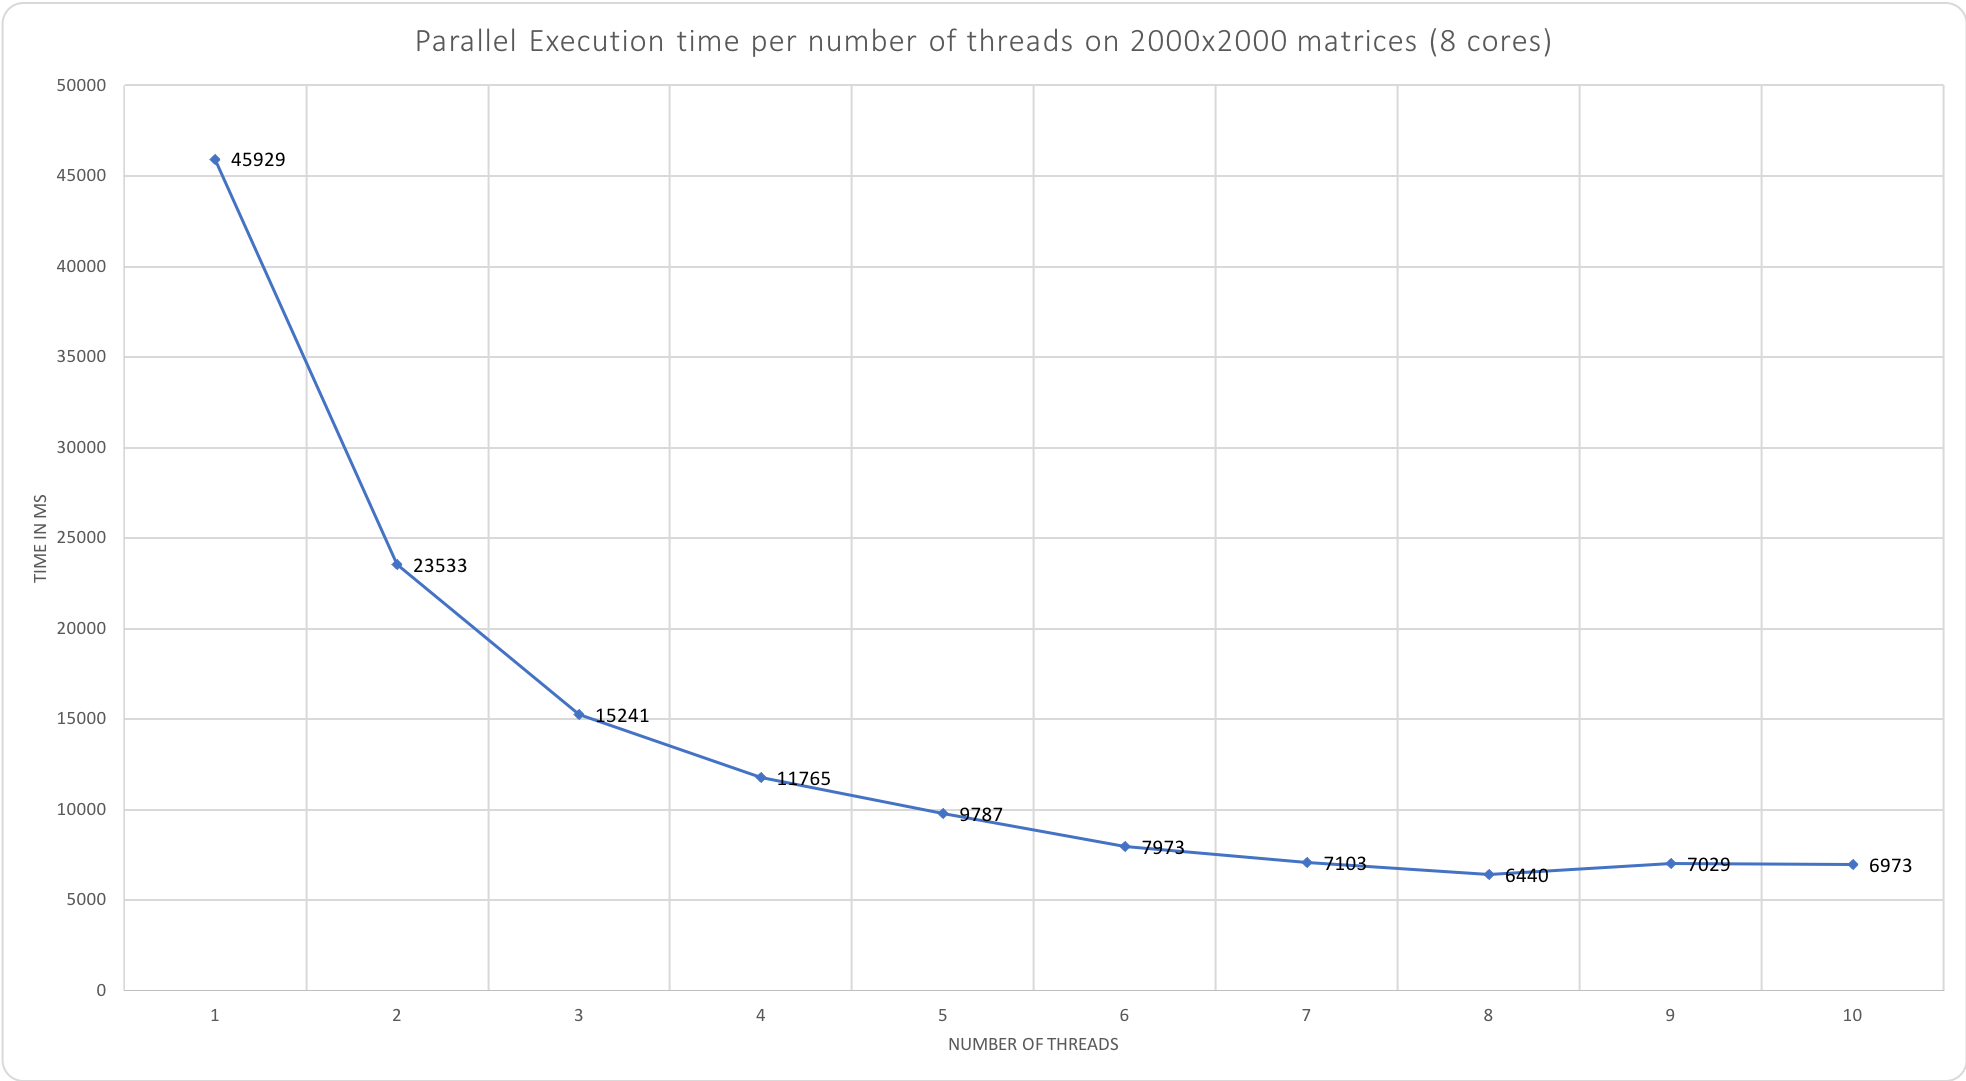
\includegraphics[scale=0.5]{ExecutionTimeThread}
			\end{figure}
		
			This graph follows an exponential decrease in resolution time as we increase the number of threads. It is important to note that we run this test on a 8 corr CPU machine. The reason for that exponential decrease is that at first the amount of work done by a single thread x becomes x/2 then x/3 and so on. The size of the region that each thread needs to calculate gets reduced by a smaller and smaller ratio every time we add a new thread. This is why the decrease in running time is exponential as the size calculated by each thread decreases by a smaller amount each time.
			
			\quad Since we are running on an 8 core machine it is normal to see a slight increase it running time when the number of threads exceeds the number of core as this adds overhead transitions cost between threads. In our case this was observed for 9 threads however for 10 threads the execution time decreased compare to the one with 9 threads. We think that this may be due to the fact that the execution region of each thread became so small that most thread managed to finish before the algorithm asked for a thread shift in the CPU which makes overhead costs less costly as we do not need to load the thread back after the switch.
			
			\begin{figure}[h!]
				\centering
				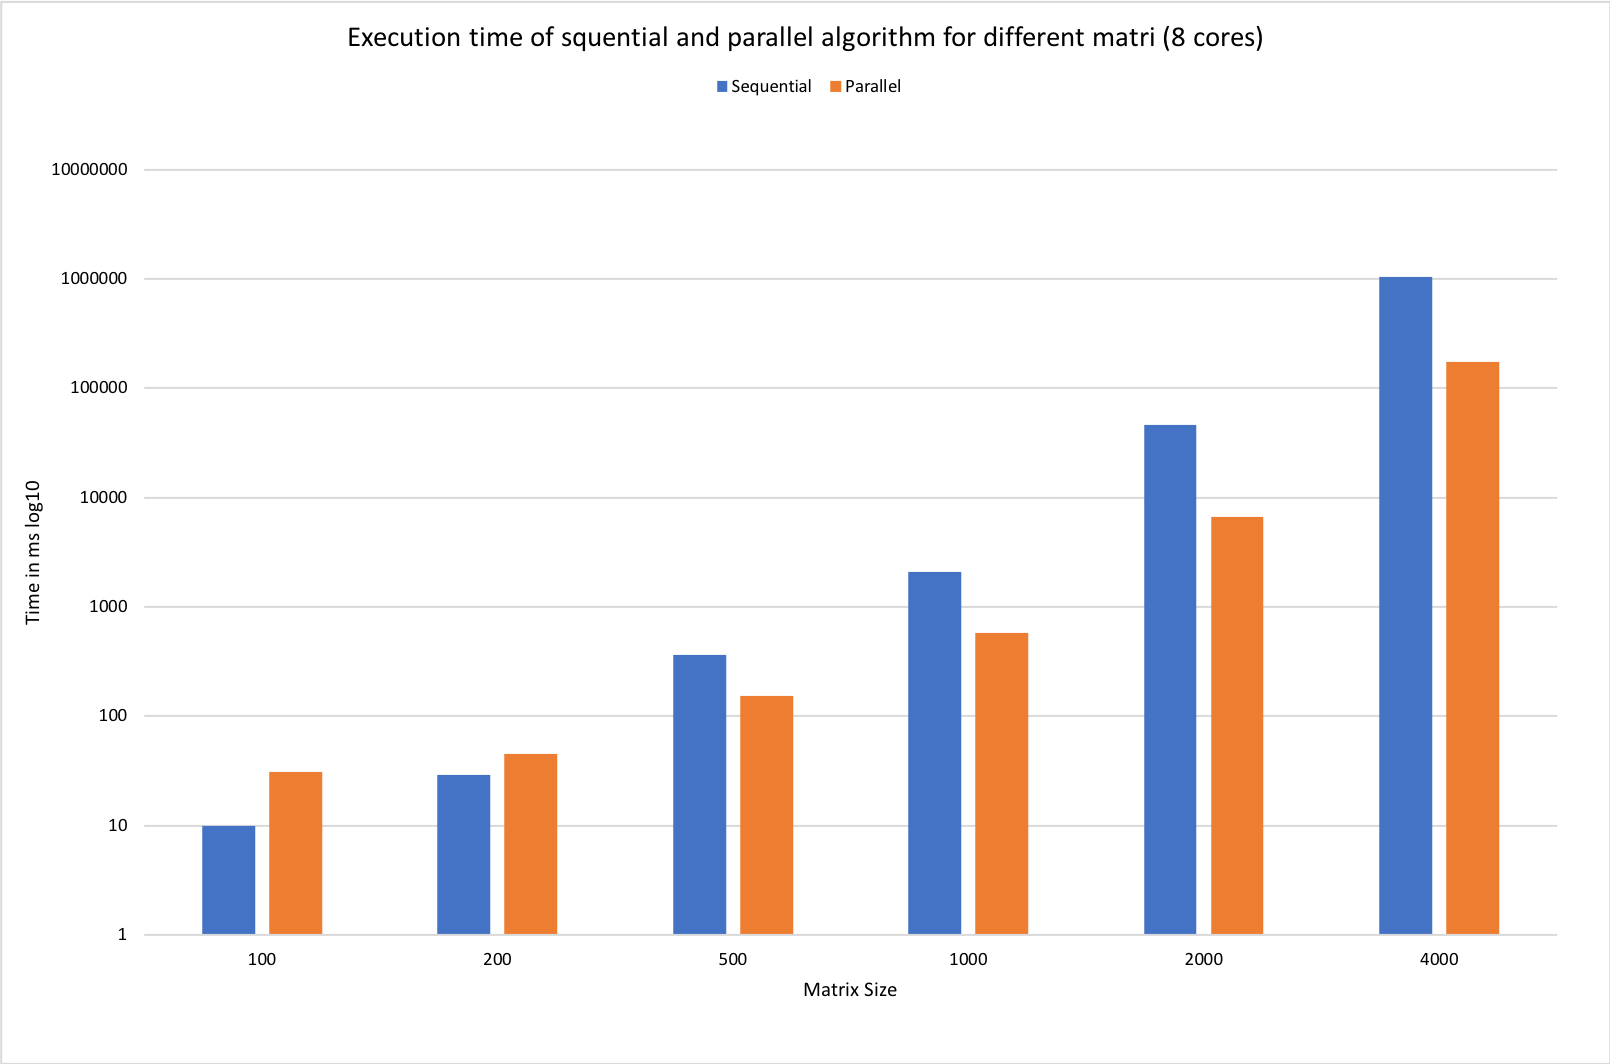
\includegraphics[scale=0.5]{ExectionParallelSequential}
			\end{figure}
			In this case we decided to graph the results on a log scale as the execution time difference between matrix size 100 and 4000 was too large to be visualized on a normal scale. Here the execution time followed a exponential increase for both parallel and sequential. In this case we can see that the execution time of sequential matrix multiplication performed better than the parallel for size 100 and 200 (note that we tried to use 1 to 8 threads for parallel and all times where worse than sequential for all combination at these matrix sizes). We think this is due to the time required to instantiate the executor and the parallelMultiplication class instantiation for parallel that adds greater overheads than just directly starting the sequential execution. However the costs of these overheads has less impact as soon as the matrix size goes over 200 here the parallel execution despite the overheads performs better.
		\question
			\begin{parts}
				\part
					In our case deadlock can occur when the sleep time of Thread 1 is longer than than the sleep time of thread 2. Since Thread 1 would have acquired the first lock but will want to acquire the second lock. Which would have already been acquired by the second thread as it walk up earlier which will be waiting to acquire the first lock. Hence we are in a deadlock as neither thread is willing to give up there lock but cannot finish there execution without the other thread's lock.
				\part
%					In our case there are different solutions to avoid that kind of deadlock. One would be to force any method in a thread willing to access locks to either access all of them at once, or if one of them cannot be accessed release all its held locks and try again. In our case this could be implemented by the tryLock() function.
					
					Hold-and-wait
					
					Require a process to request all of its required resources at a time making it block otherwise only activating it when all the resources are available. This prohibits resources from being use optimally. Sometimes it is hard to know in advance all the resources that a process will need. The programmer will have to give all the possible resources required by the process note that these are possible not required.
					
					No preemption
					
					If a process holding resources is denied a further request that process must release all its unused resources and request them again.
					
					Circular wait
					
					Can be prevented by defining a linear ordering of resource type. If a process ahs been allocated resource of type R, then it may subsequently request only those resources of types following R in the ordering. So P1 holds are R1 so it can only request $Ri>1$, P2 holds R2 so it can only request $Ri>2$. 
			\end{parts}
		
	\end{questions}
\end{document}
